\documentclass{article}
\usepackage{hyperref}
\usepackage{xcolor}
\usepackage{listings}	
\usepackage{amsmath}
\usepackage{subcaption}
\usepackage{graphicx}
\usepackage{geometry}
 \geometry{
 a4paper,
 total={170mm,257mm},
 left=10mm,
 right=10mm,
 top=10mm,
 }

\usepackage{tikz,ifthen}
\usetikzlibrary{calc}
\usetikzlibrary{intersections,perspective,decorations.pathreplacing,math}

\newcommand\downbrow[2]{
  \coordinate (a) at ( #1, #2 );
  \draw (a) -- ($ (a) + (0.2,-0.4) $) -- ($ (a) + (0.8,-0.4) $) -- ($ (a) + (1,0) $);
}

\newcommand\upbrow[2]{
  \coordinate (a) at ( #1, #2 );
  \draw (a) -- ($ (a) + (0.2,0.4) $) -- ($ (a) + (0.8,0.4) $) -- ($ (a) + (1,0) $);
}

\newcommand\rightbrow[2]{
  \coordinate (a) at ( #1, #2 );
  \draw (a) -- ($ (a) + (0.4,0.2) $) -- ($ (a) + (0.4,0.8) $) -- ($ (a) + (0,1) $);
}

\newcommand\leftbrow[2]{
  \coordinate (a) at ( #1, #2 );
  \draw (a) -- ($ (a) + (-0.4,0.2) $) -- ($ (a) + (-0.4,0.8) $) -- ($ (a) + (0,1) $);
}


\newcommand\simplecuboid[7]{
  \draw[fill=#7!80!white,opacity=0.9]
    (tpp cs:x=#1,    y=#2,    z=#3+#6) -- 
    (tpp cs:x=#1,    y=#2+#5, z=#3+#6) --
    (tpp cs:x=#1+#4, y=#2+#5, z=#3+#6) --
    (tpp cs:x=#1+#4, y=#2,    z=#3+#6) -- cycle;
  \draw[fill=#7,opacity=0.9] % Left panel
    (tpp cs:x=#1, y=#2,    z=#3)    -- 
    (tpp cs:x=#1, y=#2,    z=#3+#6) --
    (tpp cs:x=#1, y=#2+#5, z=#3+#6) --
    (tpp cs:x=#1, y=#2+#5, z=#3)    -- cycle;
  \draw[fill=#7!50!white,opacity=0.9]
    (tpp cs:x=#1,    y=#2, z=#3)    --
    (tpp cs:x=#1,    y=#2, z=#3+#6) --
    (tpp cs:x=#1+#4, y=#2, z=#3+#6) --
    (tpp cs:x=#1+#4, y=#2, z=#3)    -- cycle;
}

\title{Complementary material for kids (and curious adults too)}
\author{\href{https://github.com/cal-rmedina}{cal-rmedina}}
\date{}
\begin{document}
\maketitle

The following sections give an geometrical interpretation of the square sum,
for the series $1^2+2^2+\dots +n^2$, there is a formula for the sum of the
first $n$ terms:

\begin{equation*}
  \sum\limits_{i=1}^{n}i^2 = \dfrac{n\left(n+1\right)\left(2n+1\right)}{6}.
\end{equation*}

Each term of the series can be seen as pyramid level (Fig. \ref{fig:pyramid}), it will
help to give a geometrical interpretation to the sum, because
$n\left(n+1\right)\left(2n+1\right)$ can be seen as a square prism of size
$n \times \left(n+1\right) \times \left(2n+1\right)$.

\begin{figure}[h]
  \centering
  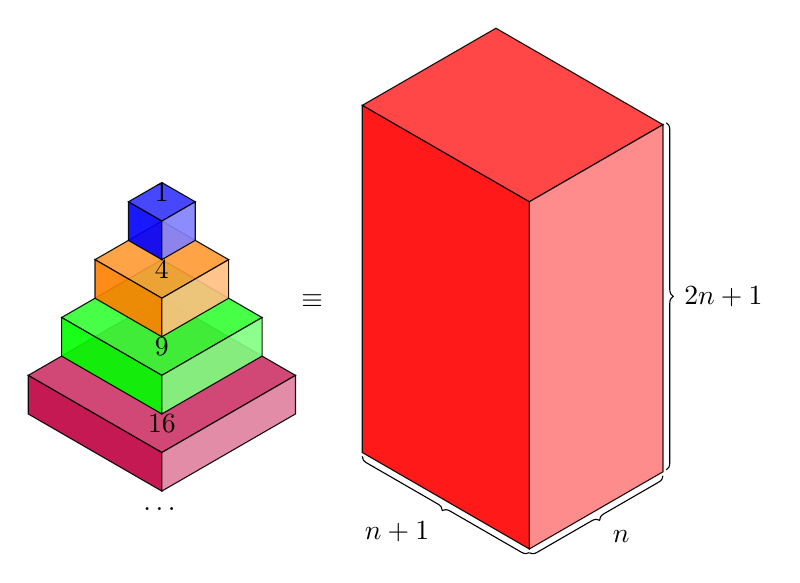
\begin{tikzpicture}[isometric view,scale=0.6]
  
    \simplecuboid{0}{0}{0}{4}{4}{1}{purple}
    \simplecuboid{1}{1}{1}{3}{3}{1}{green}
    \simplecuboid{2}{2}{2}{2}{2}{1}{orange}
    \simplecuboid{3}{3}{3}{1}{1}{1}{blue}
  
    \node[label=above:$ 16 $] at (0,0,1){};
    \node[label=above:$ 9 $] at (1,1,2){};
    \node[label=above:$ 4 $] at (2,2,3){};
    \node[label=above:$ 1 $] at (3,3,4){};

    \node[label=above:$ \dots $] at (-1,-1,0){};

    \node[label=above:$\equiv$] at (5.5,1,1){};
  
    \simplecuboid{11}{0}{-7}{4}{5}{9}{red}
  
    \draw [decorate,decoration = {brace,mirror}] (15.1,0,-7) -- (15.1,0,2)
      node[pos=0.5,right=3,black]{$2n+1$};
    \draw [decorate,decoration = {brace,mirror}] (11,0,-7.1) -- (15,0,-7.1)
      node[pos=0.5,below right=2.5,black]{$n$};
    \draw [decorate,decoration = {brace,mirror}] (11,5,-7.1) -- (11,0,-7.1)
      node[pos=0.5,below left=2.5,black]{$n+1$};

  \end{tikzpicture}
  \caption{Each box represents a term in the series
  $\textcolor{blue}{1^2} + \textcolor{orange}{2^2} + \textcolor{green}{3^2} +
  \textcolor{purple}{4^2} \dots$} \label{fig:pyramid}
\end{figure}

The pyramid \textbf{fits exactly $\mathbf{6}$ times} inside the square prism, cut-out
material is provided to check the cases $n=2,3$, the trivial case for $n=1$
won't be discussed, for a formal mathematical proof go to the
\href{https://proofwiki.org/wiki/Sum_of_Sequence_of_Squares}{link}.

\section*{Two and three terms of the sum}

Fig. \ref{fig:pyramids} serves for the geometrical proof, check
\hyperref[sec:assets]{Assets}, print and cut out the figures to construct the
square prism. 

\begin{figure}[h]
  \centering
  \begin{subfigure}[t]{0.46\textwidth}
    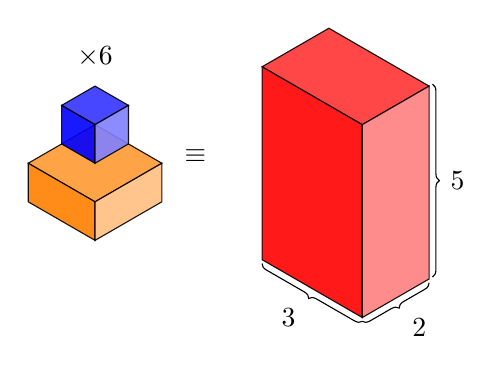
\begin{tikzpicture}[isometric view,scale=0.6]
    
      \simplecuboid{0}{0}{0}{2}{2}{1}{orange}
      \simplecuboid{1}{1}{1}{1}{1}{1}{blue}
    
      \node[label=above:$\times 6$] at (2,2,2){};
      \node[label=above:$\equiv$] at (4,1,-1){};
    
      \simplecuboid{8}{0}{-6}{2}{3}{5}{red}
    
      \draw [decorate,decoration = {brace,mirror}] (10.1,0,-6) -- (10.1,0,-1)
        node[pos=0.5,right=3,black]{$5$};
      \draw [decorate,decoration = {brace,mirror}] (8,0,-6.1) -- (10,0,-6.1)
        node[pos=0.5,below right=2.5,black]{$2$};
      \draw [decorate,decoration = {brace,mirror}] (8,3,-6.1) -- (8,0,-6.1)
        node[pos=0.5,below left=2.5,black]{$3$};
    
    \end{tikzpicture}
    \caption{$\textcolor{blue}{1^2}+\textcolor{orange}{2^2} = \textcolor{red}{5}$}
    \label{fig:p2}
  \end{subfigure}
  \hfill
  \begin{subfigure}[t]{0.46\textwidth}
    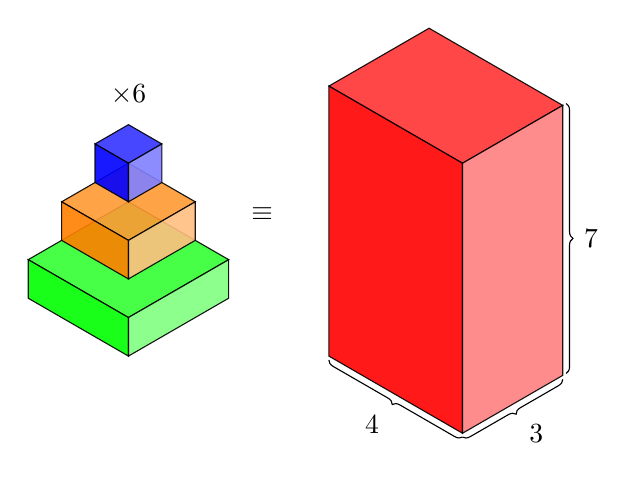
\begin{tikzpicture}[isometric view,scale=0.6]
      \simplecuboid{0}{0}{0}{3}{3}{1}{green}
      \simplecuboid{1}{1}{1}{2}{2}{1}{orange}
      \simplecuboid{2}{2}{2}{1}{1}{1}{blue}
    
      \node[label=above:$\times 6$] at (3,3,3){};
      \node[label=above:$\equiv$] at (5,1,0){};
   
      \simplecuboid{10}{0}{-7}{3}{4}{7}{red}
    
      \draw [decorate,decoration = {brace,mirror}] (13.1,0,-7) -- (13.1,0,0)
        node[pos=0.5,right=3,black]{$7$};
      \draw [decorate,decoration = {brace,mirror}] (10,0,-7.1) -- (13,0,-7.1)
        node[pos=0.5,below right=2.5,black]{$3$};
      \draw [decorate,decoration = {brace,mirror}] (10,4,-7.1) -- (10,0,-7.1)
        node[pos=0.5,below left=2.5,black]{$4$};
    
    \end{tikzpicture}
    \caption{$\textcolor{blue}{1^2}+\textcolor{orange}{2^2}+\textcolor{green}{3^2} = \textcolor{red}{14}$}
    \label{fig:p3}
  \end{subfigure}

\caption{6 pyramids build a square prism; (\ref{fig:p2}) for $n=2$ and (\ref{fig:p3}) for $n=3$.}
\label{fig:pyramids}
\end{figure}

\section*{Assets}\label{sec:assets}

\begin{figure}[h]
  \centering
  \begin{subfigure}{0.4\textwidth}
    \centering
    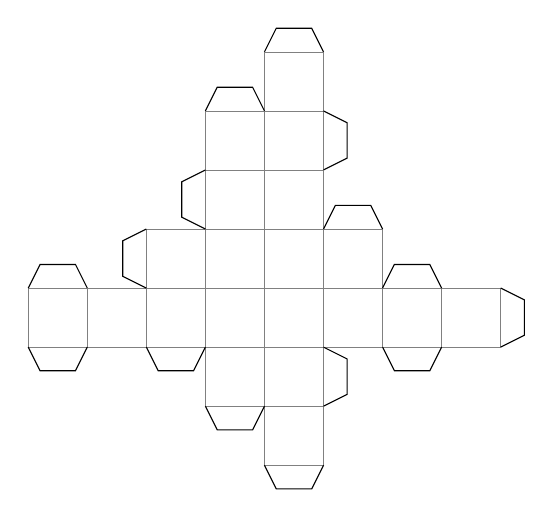
\begin{tikzpicture}[scale=0.75]
      \draw[step=1cm,gray,very thin] (4,0) grid (5,1);
      \draw[step=1cm,gray,very thin] (3,1) grid (5,2);
      \draw[step=1cm,gray,very thin] (0,2) grid (8,3);
      \draw[step=1cm,gray,very thin] (2,3) grid (6,4);
      \draw[step=1cm,gray,very thin] (3,4) grid (5,6);
      \draw[step=1cm,gray,very thin] (4,6) grid (5,7);
  
      \downbrow{0}{2}
      \downbrow{2}{2}
      \downbrow{3}{1}
      \downbrow{4}{0}
      \downbrow{6}{2}
  
      \upbrow{0}{3}
      \upbrow{3}{6}
      \upbrow{4}{7}
      \upbrow{5}{4}
      \upbrow{6}{3}
  
      \rightbrow{5}{1}
      \rightbrow{8}{2}
      \rightbrow{5}{5}
  
      \leftbrow{2}{3}
      \leftbrow{3}{4}
  
    \end{tikzpicture}
  \end{subfigure}
  \hfill
  \begin{subfigure}{0.4\textwidth}
    \centering
    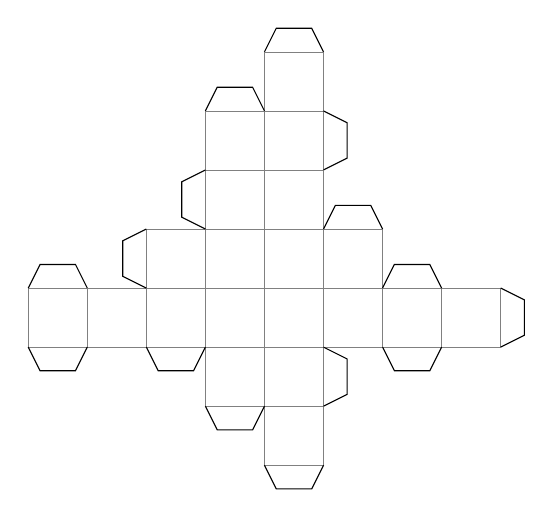
\begin{tikzpicture}[scale=0.75]
      \draw[step=1cm,gray,very thin] (4,0) grid (5,1);
      \draw[step=1cm,gray,very thin] (3,1) grid (5,2);
      \draw[step=1cm,gray,very thin] (0,2) grid (8,3);
      \draw[step=1cm,gray,very thin] (2,3) grid (6,4);
      \draw[step=1cm,gray,very thin] (3,4) grid (5,6);
      \draw[step=1cm,gray,very thin] (4,6) grid (5,7);
  
      \downbrow{0}{2}
      \downbrow{2}{2}
      \downbrow{3}{1}
      \downbrow{4}{0}
      \downbrow{6}{2}
  
      \upbrow{0}{3}
      \upbrow{3}{6}
      \upbrow{4}{7}
      \upbrow{5}{4}
      \upbrow{6}{3}
  
      \rightbrow{5}{1}
      \rightbrow{8}{2}
      \rightbrow{5}{5}
  
      \leftbrow{2}{3}
      \leftbrow{3}{4}
  
    \end{tikzpicture}
  \end{subfigure}

\end{figure}
\begin{figure}[h]
  \centering
  \begin{subfigure}{0.4\textwidth}
    \centering
    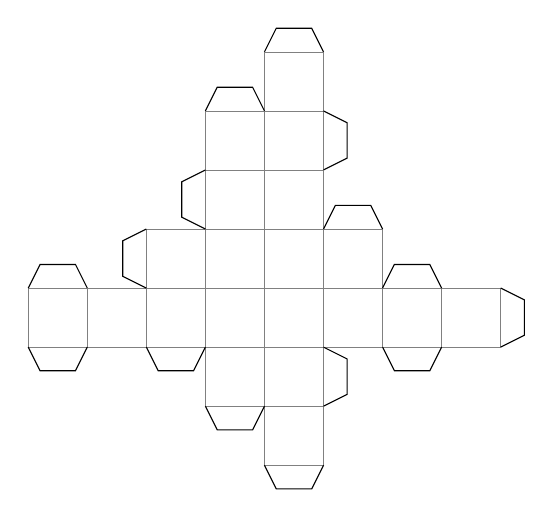
\begin{tikzpicture}[scale=0.75]
      \draw[step=1cm,gray,very thin] (4,0) grid (5,1);
      \draw[step=1cm,gray,very thin] (3,1) grid (5,2);
      \draw[step=1cm,gray,very thin] (0,2) grid (8,3);
      \draw[step=1cm,gray,very thin] (2,3) grid (6,4);
      \draw[step=1cm,gray,very thin] (3,4) grid (5,6);
      \draw[step=1cm,gray,very thin] (4,6) grid (5,7);
  
      \downbrow{0}{2}
      \downbrow{2}{2}
      \downbrow{3}{1}
      \downbrow{4}{0}
      \downbrow{6}{2}
  
      \upbrow{0}{3}
      \upbrow{3}{6}
      \upbrow{4}{7}
      \upbrow{5}{4}
      \upbrow{6}{3}
  
      \rightbrow{5}{1}
      \rightbrow{8}{2}
      \rightbrow{5}{5}
  
      \leftbrow{2}{3}
      \leftbrow{3}{4}
  
    \end{tikzpicture}
  \end{subfigure}
  \hfill
  \begin{subfigure}{0.4\textwidth}
    \centering
    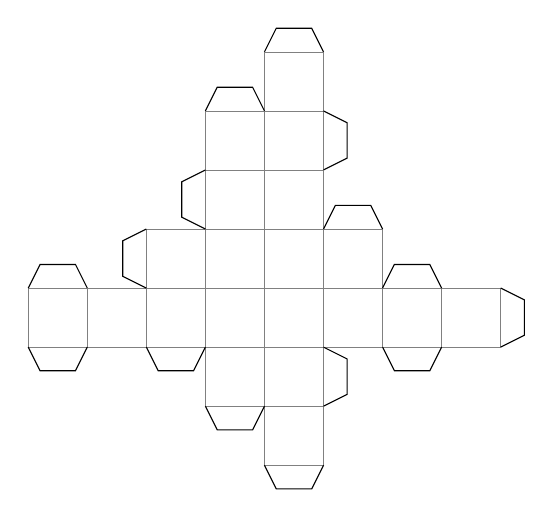
\begin{tikzpicture}[scale=0.75]
      \draw[step=1cm,gray,very thin] (4,0) grid (5,1);
      \draw[step=1cm,gray,very thin] (3,1) grid (5,2);
      \draw[step=1cm,gray,very thin] (0,2) grid (8,3);
      \draw[step=1cm,gray,very thin] (2,3) grid (6,4);
      \draw[step=1cm,gray,very thin] (3,4) grid (5,6);
      \draw[step=1cm,gray,very thin] (4,6) grid (5,7);
  
      \downbrow{0}{2}
      \downbrow{2}{2}
      \downbrow{3}{1}
      \downbrow{4}{0}
      \downbrow{6}{2}
  
      \upbrow{0}{3}
      \upbrow{3}{6}
      \upbrow{4}{7}
      \upbrow{5}{4}
      \upbrow{6}{3}
  
      \rightbrow{5}{1}
      \rightbrow{8}{2}
      \rightbrow{5}{5}
  
      \leftbrow{2}{3}
      \leftbrow{3}{4}
  
    \end{tikzpicture}
  \end{subfigure}

\end{figure}
\begin{figure}[h]
  \centering
  \begin{subfigure}{0.4\textwidth}
    \centering
    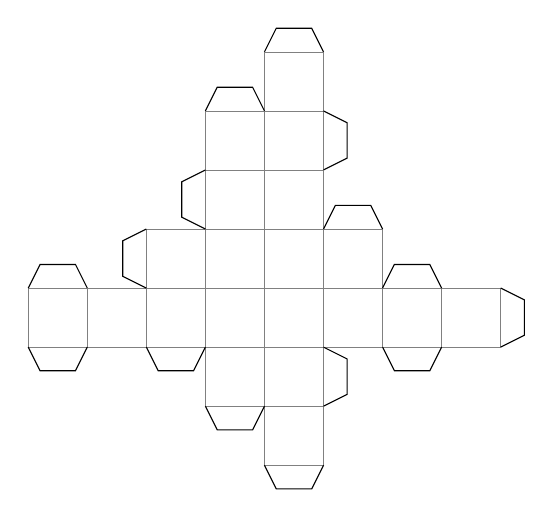
\begin{tikzpicture}[scale=0.75]
      \draw[step=1cm,gray,very thin] (4,0) grid (5,1);
      \draw[step=1cm,gray,very thin] (3,1) grid (5,2);
      \draw[step=1cm,gray,very thin] (0,2) grid (8,3);
      \draw[step=1cm,gray,very thin] (2,3) grid (6,4);
      \draw[step=1cm,gray,very thin] (3,4) grid (5,6);
      \draw[step=1cm,gray,very thin] (4,6) grid (5,7);
  
      \downbrow{0}{2}
      \downbrow{2}{2}
      \downbrow{3}{1}
      \downbrow{4}{0}
      \downbrow{6}{2}
  
      \upbrow{0}{3}
      \upbrow{3}{6}
      \upbrow{4}{7}
      \upbrow{5}{4}
      \upbrow{6}{3}
  
      \rightbrow{5}{1}
      \rightbrow{8}{2}
      \rightbrow{5}{5}
  
      \leftbrow{2}{3}
      \leftbrow{3}{4}
  
    \end{tikzpicture}
  \end{subfigure}
  \hfill
  \begin{subfigure}{0.4\textwidth}
    \centering
    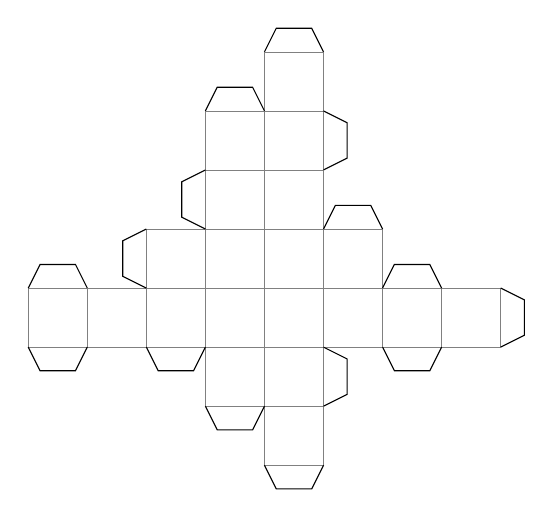
\begin{tikzpicture}[scale=0.75]
      \draw[step=1cm,gray,very thin] (4,0) grid (5,1);
      \draw[step=1cm,gray,very thin] (3,1) grid (5,2);
      \draw[step=1cm,gray,very thin] (0,2) grid (8,3);
      \draw[step=1cm,gray,very thin] (2,3) grid (6,4);
      \draw[step=1cm,gray,very thin] (3,4) grid (5,6);
      \draw[step=1cm,gray,very thin] (4,6) grid (5,7);
  
      \downbrow{0}{2}
      \downbrow{2}{2}
      \downbrow{3}{1}
      \downbrow{4}{0}
      \downbrow{6}{2}
  
      \upbrow{0}{3}
      \upbrow{3}{6}
      \upbrow{4}{7}
      \upbrow{5}{4}
      \upbrow{6}{3}
  
      \rightbrow{5}{1}
      \rightbrow{8}{2}
      \rightbrow{5}{5}
  
      \leftbrow{2}{3}
      \leftbrow{3}{4}
  
    \end{tikzpicture}
  \end{subfigure}

\end{figure}

\newpage

\begin{figure}[h]
  \centering
  \begin{subfigure}{0.4\textwidth}
    \centering
    \begin{tikzpicture}[scale=0.75]
      \draw[step=1cm,gray,very thin] (3,0) grid (4,1);
      \draw[step=1cm,gray,very thin] (3,1) grid (5,2);
      \draw[step=1cm,gray,very thin] (3,2) grid (6,3);
      \draw[step=1cm,gray,very thin] (0,3) grid (12,4);
      \draw[step=1cm,gray,very thin] (1,4) grid (9,5);
      \draw[step=1cm,gray,very thin] (2,5) grid (7,6);
      \draw[step=1cm,gray,very thin] (3,6) grid (6,8);
      \draw[step=1cm,gray,very thin] (3,8) grid (5,10);
      \draw[step=1cm,gray,very thin] (3,10) grid (4,11);
    
      \downbrow{3}{0}
      \downbrow{4}{1}
      \downbrow{5}{2}
      \downbrow{6}{3}
      \downbrow{8}{3}
      \downbrow{10}{3}
    
      \upbrow{0}{4}
      \upbrow{1}{5}
      \upbrow{2}{6}
      \upbrow{3}{11}
      \upbrow{4}{10}
      \upbrow{10}{4}
      \upbrow{7}{5}
      \upbrow{6}{6}
    
      \rightbrow{12}{3}
      \rightbrow{9}{4}
      \rightbrow{6}{7}
      \rightbrow{5}{8}
    
      \leftbrow{3}{7}
      \leftbrow{3}{9}
    
      \coordinate (a) at (0,3);
      \draw (a) -- ($ (a) + (0.2,-0.4) $) -- ($ (a) + (2.8,-0.4) $) -- ($ (a) + (3,0) $);

    \end{tikzpicture}
  \end{subfigure}

  \hfill

  \begin{subfigure}{0.4\textwidth}
    \centering
    \begin{tikzpicture}[scale=0.75]
      \draw[step=1cm,gray,very thin] (3,0) grid (4,1);
      \draw[step=1cm,gray,very thin] (3,1) grid (5,2);
      \draw[step=1cm,gray,very thin] (3,2) grid (6,3);
      \draw[step=1cm,gray,very thin] (0,3) grid (12,4);
      \draw[step=1cm,gray,very thin] (1,4) grid (9,5);
      \draw[step=1cm,gray,very thin] (2,5) grid (7,6);
      \draw[step=1cm,gray,very thin] (3,6) grid (6,8);
      \draw[step=1cm,gray,very thin] (3,8) grid (5,10);
      \draw[step=1cm,gray,very thin] (3,10) grid (4,11);
    
      \downbrow{3}{0}
      \downbrow{4}{1}
      \downbrow{5}{2}
      \downbrow{6}{3}
      \downbrow{8}{3}
      \downbrow{10}{3}
    
      \upbrow{0}{4}
      \upbrow{1}{5}
      \upbrow{2}{6}
      \upbrow{3}{11}
      \upbrow{4}{10}
      \upbrow{10}{4}
      \upbrow{7}{5}
      \upbrow{6}{6}
    
      \rightbrow{12}{3}
      \rightbrow{9}{4}
      \rightbrow{6}{7}
      \rightbrow{5}{8}
    
      \leftbrow{3}{7}
      \leftbrow{3}{9}
    
      \coordinate (a) at (0,3);
      \draw (a) -- ($ (a) + (0.2,-0.4) $) -- ($ (a) + (2.8,-0.4) $) -- ($ (a) + (3,0) $);

    \end{tikzpicture}
  \end{subfigure}
  \hfill

  \begin{subfigure}{0.4\textwidth}
    \centering
    \begin{tikzpicture}[scale=0.75]
      \draw[step=1cm,gray,very thin] (3,0) grid (4,1);
      \draw[step=1cm,gray,very thin] (3,1) grid (5,2);
      \draw[step=1cm,gray,very thin] (3,2) grid (6,3);
      \draw[step=1cm,gray,very thin] (0,3) grid (12,4);
      \draw[step=1cm,gray,very thin] (1,4) grid (9,5);
      \draw[step=1cm,gray,very thin] (2,5) grid (7,6);
      \draw[step=1cm,gray,very thin] (3,6) grid (6,8);
      \draw[step=1cm,gray,very thin] (3,8) grid (5,10);
      \draw[step=1cm,gray,very thin] (3,10) grid (4,11);
    
      \downbrow{3}{0}
      \downbrow{4}{1}
      \downbrow{5}{2}
      \downbrow{6}{3}
      \downbrow{8}{3}
      \downbrow{10}{3}
    
      \upbrow{0}{4}
      \upbrow{1}{5}
      \upbrow{2}{6}
      \upbrow{3}{11}
      \upbrow{4}{10}
      \upbrow{10}{4}
      \upbrow{7}{5}
      \upbrow{6}{6}
    
      \rightbrow{12}{3}
      \rightbrow{9}{4}
      \rightbrow{6}{7}
      \rightbrow{5}{8}
    
      \leftbrow{3}{7}
      \leftbrow{3}{9}
    
      \coordinate (a) at (0,3);
      \draw (a) -- ($ (a) + (0.2,-0.4) $) -- ($ (a) + (2.8,-0.4) $) -- ($ (a) + (3,0) $);

    \end{tikzpicture}
  \end{subfigure}
\end{figure}

\newpage

\begin{figure}[h]
  \centering
  \begin{subfigure}{0.4\textwidth}
    \centering
    \begin{tikzpicture}[scale=0.75]
      \draw[step=1cm,gray,very thin] (3,0) grid (4,1);
      \draw[step=1cm,gray,very thin] (3,1) grid (5,2);
      \draw[step=1cm,gray,very thin] (3,2) grid (6,3);
      \draw[step=1cm,gray,very thin] (0,3) grid (12,4);
      \draw[step=1cm,gray,very thin] (1,4) grid (9,5);
      \draw[step=1cm,gray,very thin] (2,5) grid (7,6);
      \draw[step=1cm,gray,very thin] (3,6) grid (6,8);
      \draw[step=1cm,gray,very thin] (3,8) grid (5,10);
      \draw[step=1cm,gray,very thin] (3,10) grid (4,11);
    
      \downbrow{3}{0}
      \downbrow{4}{1}
      \downbrow{5}{2}
      \downbrow{6}{3}
      \downbrow{8}{3}
      \downbrow{10}{3}
    
      \upbrow{0}{4}
      \upbrow{1}{5}
      \upbrow{2}{6}
      \upbrow{3}{11}
      \upbrow{4}{10}
      \upbrow{10}{4}
      \upbrow{7}{5}
      \upbrow{6}{6}
    
      \rightbrow{12}{3}
      \rightbrow{9}{4}
      \rightbrow{6}{7}
      \rightbrow{5}{8}
    
      \leftbrow{3}{7}
      \leftbrow{3}{9}
    
      \coordinate (a) at (0,3);
      \draw (a) -- ($ (a) + (0.2,-0.4) $) -- ($ (a) + (2.8,-0.4) $) -- ($ (a) + (3,0) $);

    \end{tikzpicture}
  \end{subfigure}

  \hfill

  \begin{subfigure}{0.4\textwidth}
    \centering
    \begin{tikzpicture}[scale=0.75]
      \draw[step=1cm,gray,very thin] (3,0) grid (4,1);
      \draw[step=1cm,gray,very thin] (3,1) grid (5,2);
      \draw[step=1cm,gray,very thin] (3,2) grid (6,3);
      \draw[step=1cm,gray,very thin] (0,3) grid (12,4);
      \draw[step=1cm,gray,very thin] (1,4) grid (9,5);
      \draw[step=1cm,gray,very thin] (2,5) grid (7,6);
      \draw[step=1cm,gray,very thin] (3,6) grid (6,8);
      \draw[step=1cm,gray,very thin] (3,8) grid (5,10);
      \draw[step=1cm,gray,very thin] (3,10) grid (4,11);
    
      \downbrow{3}{0}
      \downbrow{4}{1}
      \downbrow{5}{2}
      \downbrow{6}{3}
      \downbrow{8}{3}
      \downbrow{10}{3}
    
      \upbrow{0}{4}
      \upbrow{1}{5}
      \upbrow{2}{6}
      \upbrow{3}{11}
      \upbrow{4}{10}
      \upbrow{10}{4}
      \upbrow{7}{5}
      \upbrow{6}{6}
    
      \rightbrow{12}{3}
      \rightbrow{9}{4}
      \rightbrow{6}{7}
      \rightbrow{5}{8}
    
      \leftbrow{3}{7}
      \leftbrow{3}{9}
    
      \coordinate (a) at (0,3);
      \draw (a) -- ($ (a) + (0.2,-0.4) $) -- ($ (a) + (2.8,-0.4) $) -- ($ (a) + (3,0) $);

    \end{tikzpicture}
  \end{subfigure}
  \hfill

  \begin{subfigure}{0.4\textwidth}
    \centering
    \begin{tikzpicture}[scale=0.75]
      \draw[step=1cm,gray,very thin] (3,0) grid (4,1);
      \draw[step=1cm,gray,very thin] (3,1) grid (5,2);
      \draw[step=1cm,gray,very thin] (3,2) grid (6,3);
      \draw[step=1cm,gray,very thin] (0,3) grid (12,4);
      \draw[step=1cm,gray,very thin] (1,4) grid (9,5);
      \draw[step=1cm,gray,very thin] (2,5) grid (7,6);
      \draw[step=1cm,gray,very thin] (3,6) grid (6,8);
      \draw[step=1cm,gray,very thin] (3,8) grid (5,10);
      \draw[step=1cm,gray,very thin] (3,10) grid (4,11);
    
      \downbrow{3}{0}
      \downbrow{4}{1}
      \downbrow{5}{2}
      \downbrow{6}{3}
      \downbrow{8}{3}
      \downbrow{10}{3}
    
      \upbrow{0}{4}
      \upbrow{1}{5}
      \upbrow{2}{6}
      \upbrow{3}{11}
      \upbrow{4}{10}
      \upbrow{10}{4}
      \upbrow{7}{5}
      \upbrow{6}{6}
    
      \rightbrow{12}{3}
      \rightbrow{9}{4}
      \rightbrow{6}{7}
      \rightbrow{5}{8}
    
      \leftbrow{3}{7}
      \leftbrow{3}{9}
    
      \coordinate (a) at (0,3);
      \draw (a) -- ($ (a) + (0.2,-0.4) $) -- ($ (a) + (2.8,-0.4) $) -- ($ (a) + (3,0) $);

    \end{tikzpicture}
  \end{subfigure}
\end{figure}

\end{document}
